%% LaTeX-Beamer template for KIT design
%% by Erik Burger, Christian Hammer
%% title picture by Klaus Krogmann
%%
%% version 2.0
%%
%% mostly compatible to KIT corporate design v2.0
%% http://intranet.kit.edu/gestaltungsrichtlinien.php
%%
%% Problems, bugs and comments to
%% burger@kit.edu

\documentclass[18pt]{beamer}
\usetheme{kit}

%% TITLE PICTURE

% if a custom picture is to be used on the title page, copy it into the 'logos'
% directory, in the line below, replace 'mypicture' with the 
% filename (without extension) and uncomment the following line
% (picture proportions: 63 : 20, *.eps format if you use latex+dvips+ps2pdf,
% *.jpg/*.png/*.pdf if you use pdflatex)

%\titleimage{mypicture}

%% TITLE LOGO

% for a custom logo on the front page, copy your file into the 'logos'
% directory, insert the filename in the line below and uncomment it

%\titlelogo{mylogo}

% (*.eps format if you use latex+dvips+ps2pdf,
% *.jpg/*.png/*.pdf if you use pdflatex)

%% BIBTEX ICON/KEY

% if you want to see BibTeX keys in the references view instead of the symbol,
% uncomment the following line
% \usebibitemtemplate{\insertbiblabel}

% the presentation starts here

% change the following line to "ngerman" for German style date and logos
% change the following line to "english" for English style date and logos
\selectlanguage{ngerman}

\beamertemplatenavigationsymbolsempty

\usepackage{listings}
\definecolor{darkgray}{rgb}{0.95,0.95,0.95}
\definecolor{darkgreen}{rgb}{0.05,0.7,0.05}
\lstset{ language=Java,
	backgroundcolor=\color{darkgray}, 
	numbers=none, 
	keywordstyle=\color{black}\bfseries,
	tabsize=2,
	showspaces=false,               % show spaces adding particular underscores
	showstringspaces=false,         % underline spaces within strings
	showtabs=false, 
}



\title[Tutorium05]{Tutorium 05: Parallelismus und Testen}
\subtitle{Softwaretechnik im SS 2011, Tutorium 4}
\author{Jürgen Walter}
\date{\today}

\institute{Chair for Software Design and Quality}

\begin{document}

%title page
\begin{frame}
\titlepage
\end{frame}

%table of contents
\frame{
\frametitle{Was machen wir heute?}
	\tableofcontents
}

\section{Altes Übungsblatt}

\subsection{Altes Übungsblatt}
\frame {
\frametitle{Altes Übungsblatt}
	\begin{block}{Aufgabe 1 - Entwurfsmuster in der Java-API}
	\begin{itemize}
	\item ???
	\end{itemize}
	\end{block}

	\begin{block}{Aufgabe 2 - Kreuzworträtsel}
	\begin{itemize} \pause
	\item geschenkte Punkte \pause
	\item der Zusammenhang zwischen der Beschreibung und dem Muster sollte euch dennoch klar werden!
	\end{itemize}
	\end{block}
}


\begin{frame}[fragile]
\frametitle{Altes Übungsblatt}
	\begin{block}{Aufgabe 3 - Entwurfsmuster anwenden}
	\begin{itemize}
	\item ???
	\end{itemize}
	\end{block}
\end{frame}


\subsection{Zum Aufwärmen ...}
\frame {
\frametitle{Wahr oder falsch?}
\begin{itemize}
	\color<2->[rgb]{1,0,0}
	\item Die letzte Phase des klassischen Wasserfallmodells ist „Testen und Abnahme“.
	\color[rgb]{0,0,0}
	\pause
	\color<3->[rgb]{0,1,0}
	\item Regressionstests helfen verhindern, dass alte Fehler wieder auftreten.
	\color[rgb]{0,0,0}
	
	\pause
	\color<4->[rgb]{1,0,0}
	\item Funktionale Attribute spezifizieren wie gut die Software ihre Funktionen erfüllt.
	\color[rgb]{0,0,0}
	\pause
	\color<5->[rgb]{0,1,0}
	\item Bei Gleichheit 0. Stufe handelt es sich um identische Objekte.
	\color[rgb]{0,0,0}
	\pause
	\color<6->[rgb]{1,0,0}
	\item In einer transparenten Schichtenarchitektur kann eine Schicht sowohl auf die nächsthöhere als auch die nächstniedrigere Schicht zugreifen
	\color[rgb]{0,0,0}

\pause
	\color<7->[rgb]{1,0,0}
	\item Bei der Anforderungsvalidierung in der Planungsphase wird nicht überprüft, ob die Anforderungen erfüllt werden können.
	\color[rgb]{0,0,0}


\end{itemize}
}

\frame {
\frametitle {Klausuraufgaben zum Aufwärmen} 
	\begin{block} {Aufgabe 1 (1P)}
Was ist der Nachteil von Zyklen in der Benutzt-Relation zwischen Modulen? \\
	\visible<2-> {
	Die einzelnen Module können nicht nacheinander implementiert
und getestet werden, weil ihr Funktionieren von einer korrekten
Implementierung aller Module des Zyklus abhängt. Oder:
„Nothing works until everything works.“
	}
	\end{block}
}

\frame {
\frametitle {Klausuraufgaben zum Aufwärmen} 
	\begin{block} {Aufgabe 2 (2P)}
Nennen Sie jeweils zwei in der Vorlesung besprochene Entwurfsmuster der Kategorien Entkopplungsmuster und Variantenmuster und ordnen Sie die genannten Entwurfsmuster der entsprechenden Kategorie zu. \\

	
	\begin{itemize}
		\item Entkopplungsmuster: 
		\visible<2-> {Adapter, Beobachter, Brücke, Iterator, Stellvertreter, Vermittler}
		\item Variantenmuster:
		\visible<3-> {Abstrakte Fabrik, Besucher, Erbauer, Fabrikmethode, Kompositum, Schablonenmethode, Strategie, Dekorierer}
	\end{itemize}
	
	\end{block}
}

\begin{frame}[fragile]
\frametitle {Klausuraufgaben zum Aufwärmen} 
	\begin{block} {Aufgabe 3 (1P)}

	\begin{lstlisting} {}
	public static double blub(double[] d) {
		if  (d != null \&\& d.length > 0) {
		...
		}
		...
	}
	\end{lstlisting}
	
	Begründen Sie: Was wäre die Folge, wenn man das \&\& durch ein \& ersetzt?
	\visible<2-> {
	Keine Kurzauswertung (0,5 P) 
	$\Rightarrow$ Bei null als Eingabe gäbe es eine NullPointerExeption bei d.length (0,5 P).
	}
	\end{block} 
\end{frame}

\frame {
\frametitle {Klausuraufgaben zum Aufwärmen} 
	\begin{block} {Aufgabe 1 (1P)}
Erklären Sie, was eine Verklemmung ist und welche Auswirkung sie hat \\
	\visible<2-> {
	\begin{itemize}
		\item Eine Blockade, die durch eine zyklische Abhängigkeit von Fäden auf Ressourcen hervorgerufen wird
		\item Eine Verklemmung führt dazu, dass alle beteiligten Fäden ewig im Wartezustand verharren
	\end{itemize}
	}
	\end{block}
}
\section{Kontrollflussorientiertes Testen}
\frame {
\frametitle{Kontrollflussorientiertes Testen}
\begin{itemize}
\item Anweisungsüberdeckung 
\item Zweigüberdeckung
\item Pfadüberdeckung 
\item Bedingungsüberdeckung
\end{itemize}
$\Rightarrow$ Werden jedoch über Kontrollflussgraphen definiert \\
$\Rightarrow$ zunächst strukturerhaltende Transformation in Zwischensprache
}

\frame {
\frametitle{Beispiel Transformation}
\begin{center}
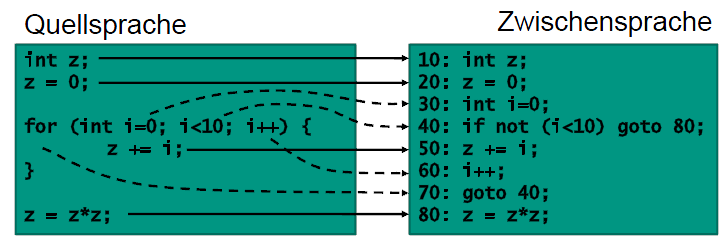
\includegraphics[scale=0.6]{pics/05/tr.png}
\end{center}

}

\frame {
\frametitle{Kontrollflussgraph}
\begin{itemize}
	\item Besteht aus Menge von Grundblöcken: Menge von Anweisungen in Zwischensprache,
		\begin{itemize}
			\item in die in die der Kontrollfluss nur am Anfang eintritt 
			\item und die außer am Ende keine Sprungbefehle enthält.
		\end{itemize}
		\item Start- und Stoppblock
		\item Menge von gerichteten Kanten, die die Ausführungsreihenfolge angeben \\
		$\Rightarrow$ Eine Kante in einem KFG wird Zweig genannt
\end{itemize}

}

\frame {
\frametitle{Beispiel KFG}
\begin{center}
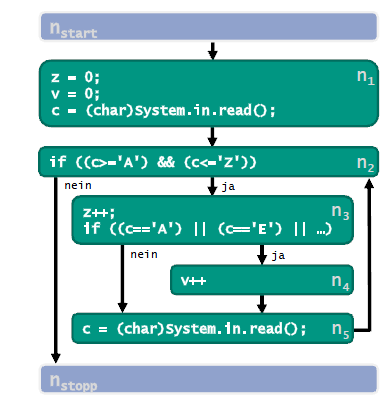
\includegraphics[scale=0.6]{pics/05/KFG.png}
\end{center}

}

\frame {
\frametitle{Teststrategien}
\begin{itemize}
\item Anweisungsüberdeckung : Ausführung aller Grundblöcke eines Programms
\item Zweigüberdeckung: Traversieren aller Zweige im KFG
\item Pfadüberdeckung : Ausführung aller unterschiedlicher Pfade im Programm

\begin{center}
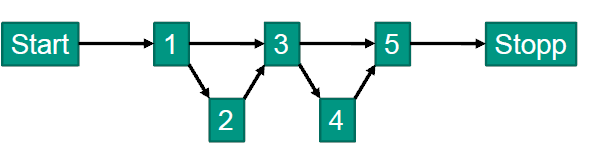
\includegraphics[scale=0.6]{pics/05/diagramm.png}
\end{center}

Anweisungs-, Zweigs-, Pfadüberdeckung?
\end{itemize}

}

\frame {
\frametitle{Aufgabe}


Gegeben sei der folgende Algorithmus, der Werte aus dem RGB-Farbraum in Werte des HSV-Farbraums umrechnet.
\begin{center}
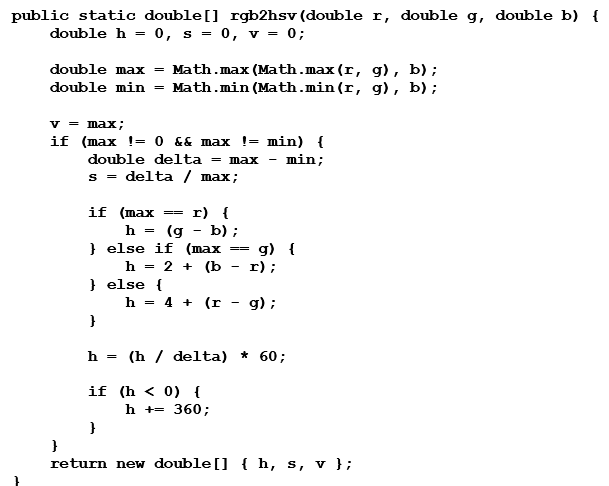
\includegraphics[scale=0.45]{pics/05/code.png}
\end{center}


}

\frame {
\frametitle{Aufgabe a)}

a) Übersetzen sie den Algorithmus in die in der Vorlesung besprochene Zwischensprache und erstellen sie daraus den Kontrollflussgraphen
\begin{center}
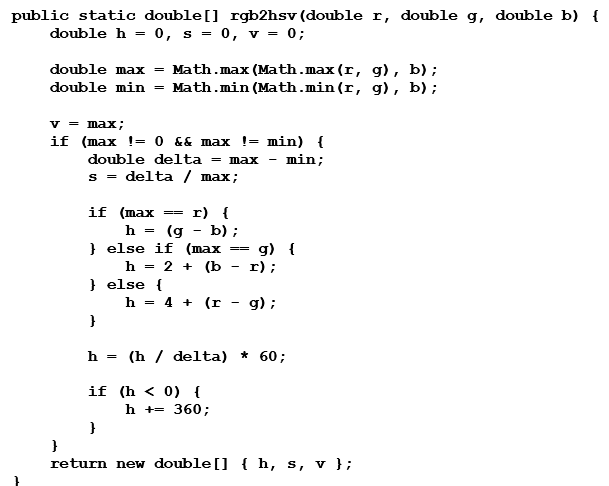
\includegraphics[scale=0.45]{pics/05/code.png}
\end{center}

}

\frame {
\frametitle {Musterlösung Teil a)}
\begin{center}
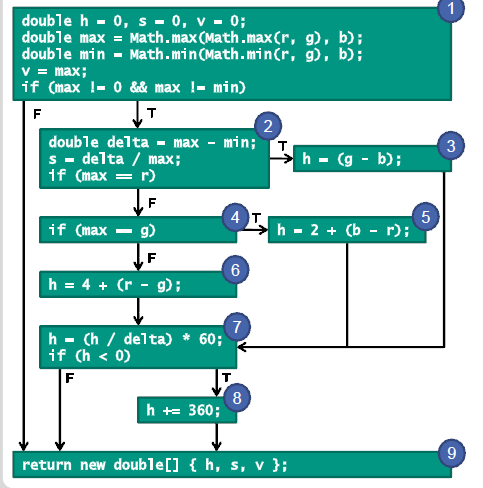
\includegraphics[scale=0.45]{pics/05/testM.png}
\end{center}
}
\frame {
\frametitle{Aufgabe Teil b )+ c))}
Für gültige Eingabewerte gilt: $r, g, b \in  [0, 1]$; für gültige Ausgaben: $s, v \in [0, 1]$ und $h \in [0, 360]$.

b) Geben Sie eine minimale Testfallmenge an, welche die Anweisungsüberdeckung erfüllt und eine, welche die Zweigüberdeckung erfüllt. 
Geben Sie für jeden Testfall den durchlaufenen Pfad im Kontrollflussgraphen an. \\
Anweisungsüberdeckung:
\visible<2-> {
 $\{1.0, 0.0, 0.5\} \rightarrow 1, 2, 3, 7, 8, 9$ $ \{0.0, 1.0, 0.0\}\rightarrow 1, 2, 4, 5, 7, 9 $ $\{0.0, 0.0, 1.0\} \rightarrow 1, 2, 4, 6, 7, 9 $
 } \\

Zweigüberdeckung:
 \visible<3-> {
siehe oben + $\{0.0, 0.0, 0.0\} \rightarrow 1, 9$ \\
}
c) Welches Problem gibt es bei der Pfadüberdeckung für diesen Algorithmus?
\visible<4-> {
Pfadüberdeckung: einige Pfade sind bei korrekten Eingaben nicht ausführbar. Wenn max $\neq$r ist, kann $h<0$ nicht wahr werden
}


}



\section{Synchronisierung}
\begin{frame}[fragile]
\frametitle {Synchronisierung} 
	\begin{block} {kritische Sektionen}

	\begin{lstlisting} {}
	private int var = 1;
	public void incorrect() {
	  if  (var > 0) {
  	    var--;
	  }
	}
	\end{lstlisting}
	
	Weshalb kann das schiefgehen? \\
	\visible<2-> {
	Falls mehrere Threads die Methode gleichzeitig aufrufen, kann einer davon die Bedingung prüfen und dann ``stehen bleiben'', während ein anderer Thread $var$ dekrementiert. \\
	}
	Lösung: \visible<3-> {den kritischen Abschnitt schützen, z.B. mit $synchronized$}
	\end{block} 
\end{frame}



\section{Ende}
\subsection{Tipps zum nächsten Übungsblatt}

\frame{
\frametitle{Tipps zum nächsten Übungsblatt}

	\begin{block}{Aufgabe 1 - Kontrollflussorientiertes Testen}
	\begin{itemize}
	\item kommt oft in der Klausur vor \pause
	\item relativ leicht verdiente Punkte!
	\end{itemize}
	\end{block}
}

\frame{
\frametitle{Tipps zum nächsten Übungsblatt}

	\begin{block}{Aufgabe 2 -Gebietszerlegung und Synchronisation}
	\begin{itemize} \pause
	\item a) sollte jeder hinbekommen - falls euch nichts einfällt wählt einfach ein paar Parameter und schaut was passiert \pause
	\item b) sieht auf den ersten Blick harmlos aus - um sicher zu gehen programmiert ein Testprogramm und testet, ob euer Fix tatsächlich das Problem behebt \pause
	\item stellt dazu auch sicher, dass die ursprüngliche Barriere tatsächlich falsch funktioniert in eurem Test-Programm \pause
	\item ein Test ist nur dann sinnvoll, wenn er den Unterschied zwischen richtigem und falschem Code auch zeigt - \pause
	\item sonst kann es sein, dass euer Test das eigentliche Fehlverhalten nicht sichtbar macht \pause
	\item Achtung: wait() kann auch ``grundlos'' enden, daher sollte wait() immer in einer Schleife stehen
	\end{itemize}
	\end{block}
}


\frame{
\frametitle{Tipps zum nächsten Übungsblatt}
	\begin{block}{Aufgabe 3 - Parallelisierung}
	\begin{itemize}
	\item für diese Aufgabe gibt es 9 ``Pflicht''- und 5 Bonuspunkte
	\item ihr braucht zum Testen einen Rechner mit mindestens zwei Kernen - \\
		falls ihr keinen habt, gibt es in der Atis genug davon (Core2Duo, Core i5, Athlon X2)
	\item zuverlässige Laufzeitmessungen kann man oft brauchen, und es gibt dabei mehr als genug Fehlerquellen ;-) \pause
	\item Zeitmessungen sind immer ungenau - die Bearbeitungszeit sollte daher nicht kürzer als eine Sekunde sein \pause
	\item das Programm soll sowohl: \\
		mit Kommandozeilenargumenten mit Hilfe von Configuration.java (wie bei ÜB2), \\ \pause
		also auch ohne Argumente mit einem GUI (wie bei ÜB3) gestartet werden können
	\end{itemize}
	\end{block}
}

\frame{
\frametitle{Tipps zum nächsten Übungsblatt}
	\begin{block}{Parallelisierungsarten}
	\begin{itemize}
	\item es gibt Programme, die ``embarassingly Parallel'' sind - indem man das Programm z.B. n-Mal mit n verschiedenen Dateien als Argument startet \pause
	\item hier soll allerdings die Bearbeitung nur $eines$ Bildes beschleunigt werden \pause
	\item sehr oft gibt es auch Datenparallelität - Berechnungen werden auf großen Datenstrukturen ausgeführt, ohne, dass es Abhängigkeiten zwischen den einzelnen Datenpunkten gibt - z.B. Matrixmultiplikation
	\end{itemize}
	\end{block}
}

\frame{
\frametitle{Tipps zum nächsten Übungsblatt}
	\begin{block}{Parallelisierungsarten}
	\begin{itemize}
	\item allgemein spricht man beim Aufteilen von Teilaufgaben von Aufgaben- bzw. Taskparallelität \pause
	\item Beispiel: es kann gleichzeitig die Summe von Vektor A und der Durschnitt von Vektor B berechnet werden \pause
	\item wenn es eine Menge aufeinanderfolgende Arbeitsschritte gibt, die jeweils unterschiedliche Ressourcen erfordern und viele Elemente diese Schritte durchlaufen sollen, bietet sich eine Pipeline an \pause
	\item zu jeder Pipelinestufe gehört (min.) ein Thread, und sobald alle Stufen fertig sind, wandern die Elemente zur jeweils nächsten Stufe
	\end{itemize}
	\end{block}
}

\frame{
\frametitle{Tipps zum nächsten Übungsblatt}
	\begin{block}{Aufgabe 3 - Parallelisierung}
	\begin{itemize}
	\item es können hier nicht alle Punkte gleichzeitig bearbeitet werden  \pause
	\item wenn ihr die Arbeitsweise des sequentiellen Algorithmus betrachtet, sollten sich Datenelemente zeigen, die gleichzeitig von verschiedenen Threads bearbeitet werden können \pause
	\item damit die einzelnen Threads genug zu tun haben, lohnt es sich evtl. Elemente in größere Blöcke zu Bündeln, wobei jeder Block von seinem eigenen Thread bearbeitet wird \pause
	\item es kann durchaus sein, dass zu Beginn und Ende der Bearbeitung nicht alle n Threads Arbeit haben \pause
	\item da ihr große Bilder verwendet, wird das nicht zu sehr ins Gewicht fallen 
	\end{itemize}
	\end{block}
}
\frame{
\frametitle{Tipps zum nächsten Übungsblatt}
	\begin{block}{Aufgabe 3 - Parallelisierung}
	\begin{itemize}

	\item als Beispiel für die Verteilung von Arbeit, könnt ihr euch in JMJRST die Klassen Producer und Consumer anschauen \pause
	\item alternativ könnten die Klassen Executors, ExecutorCompletionService, Callable und Future aus dem Paket java.util.concurrent für euch interessant sein \pause
	\item diese Klassen bieten zusätzlichen Komfort, erfordern aber auch etwas Einarbeitung \pause
	\item ein Anwendungsbeispiel dafür findet ihr in Aufgabe 5.1 vom letzten Jahr
	\end{itemize}
	\end{block}
}

\frame{
\frametitle{Bis zum nächsten Mal}
	\begin{center}
	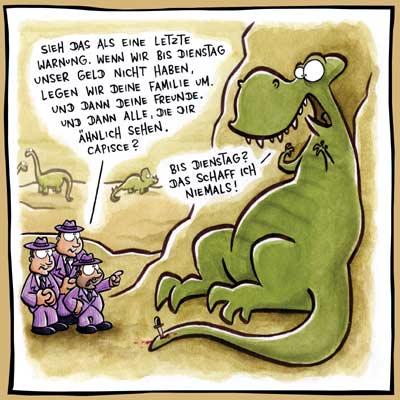
\includegraphics[height=200pt]{pics/05/05_comic}
	\end{center}
}

\end{document}
